\documentclass[11pt,a4paper]{article}
\usepackage[margin=23mm]{geometry}
\usepackage[T1]{fontenc}
\usepackage{lmodern}
\usepackage{amsmath,amssymb,booktabs,graphicx}
\usepackage[colorlinks=true,allcolors=blue]{hyperref}
\usepackage{microtype}
\makeatletter
\renewenvironment{thebibliography}[1]
{\section{Bibliography}\list{\@biblabel{\@arabic\c@enumiv}}
{\usecounter{enumiv}\setlength{\leftmargin}{2em}\setlength{\labelwidth}{1.5em}\setlength{\labelsep}{.5em}}\sloppy}
{\endlist}
\makeatother
\setlength{\parskip}{4pt}
\setlength{\parindent}{0pt}
\setlength{\emergencystretch}{1em}
\setcounter{topnumber}{3}
\setcounter{bottomnumber}{2}
\renewcommand{\topfraction}{.92}
\renewcommand{\bottomfraction}{.85}
\renewcommand{\textfraction}{.07}
\renewcommand{\floatpagefraction}{.8}
\title{Stochastic Phase-Locked Loops:\\Numerical Validation, Lock Retention and Noise-Induced Slips}
\author{}
\date{13 November 2026}
\begin{document}
\maketitle
\begin{abstract}
We investigate a textbook second-order phase-locked loop under additive Gaussian white noise. The executed study comprises 56,500 independent PLL Brownian trajectories and nine deterministic controls across a full noise--detuning grid, a separate acquisition ensemble, longer first-passage experiments, inertia/gain sensitivity and two coupled numerical-resolution ensembles. At the baseline $(\delta,\alpha)=(0.5,0.15)$, terminal phase variance is 0.0127 rad$^2$, with no committed slips observed among 1000 paths by $T=50$. At $(0.95,0.15)$, 230 transitions occur over the same horizon and 1508 occur in a separate $T=200$ ensemble. Coupled meshes support approximately first-order endpoint strong error relative to a finer numerical solution. All locking and slip statements are finite-horizon operational outcomes; neither permanent locking nor a physical hardware reproduction is claimed.
A separate 72,000-network study compares communication topologies, correlation, dropout and delay, and distinguishes phase concentration from frequency synchronization.
\end{abstract}

\section{Motivation and Background}
Phase-locked loops adjust an oscillator to track a reference phase. Noise perturbs this feedback process and can produce small fluctuations, loss of finite-time capture, or completed changes by $2\pi$ in unwrapped phase. A deterministic attracting equilibrium does not specify how often noisy paths leave its neighborhood. This project asks how detuning and noise alter these outcomes, how mesh size affects the numerical answer, and what information is lost by counting temporary threshold crossings as slips.

The starting point is the communications example in Kloeden and Platen, Chapter~7, p.~274, equation~(10.4) \cite{kloeden1992}. The supplied page image was inspected directly. The original Python script already implements the correct Euler--Maruyama recurrence under its stated unit-Wiener convention. Its five illustrative stochastic paths do not constitute an uncertainty or rare-event study. We preserve that source and reproduce its six seed settings separately, then add independent ensembles, explicit event definitions, trajectory-level uncertainty and convergence analysis. No measured hardware dataset or physical time calibration is available; the data below are simulations of the stated model.

\section{Brief Literature Survey}
Kloeden and Platen provide the model source and a general numerical SDE framework \cite{kloeden1992}. Higham distinguishes Euler--Maruyama, Milstein, strong and weak errors, and numerical stability \cite{higham2001}. These distinctions motivate coupled Brownian paths for mesh comparisons and prevent treating Monte Carlo spread as discretization error.

Bobrovsky and Schuss describe second-order PLL cycle slipping as a Kolmogorov exit problem \cite{bobrovsky1982}; their publisher abstract and metadata were verified, but their full asymptotic formula is not used here. Kramers' primary barrier-escape analysis provides the historical setting for noise-assisted transitions and damping-dependent rates \cite{kramers1940}. Khasminskii distinguishes moment, almost-sure and distributional questions of stochastic stability \cite{khasminskii2012}. No theorem number from an inaccessible text is claimed as a validation result.

Bianchi et al. demonstrate solver- and initialization-dependent errors in a different, lead--lag-filter PLL \cite{bianchi2015}. Their examples support caution about inferring global capture from a few trajectories, without establishing hidden attractors in this project. The Kuramoto review motivates a separately defined synthetic network of phase oscillators \cite{acebron2005}. Sparse LLM debate is an empirical communication baseline \cite{li2024}; it supplies no derivation that language-model messages obey PLL dynamics. GSM8K is a possible later benchmark \cite{cobbe2021,gsm8krepository}. This targeted source-checked survey is not an exhaustive statement of all literature through 2026.

\section{Model Description}
\subsection{Source equation and stochastic convention}
Write detuning as $\Delta=\omega-\omega_0$. The verified equation is
\begin{equation}
a\ddot\phi+\dot\phi+ab\sin\phi=\Delta-\alpha\zeta_t,
\qquad a>0,\ b>0,\ \alpha\ge0.
\label{eq:second}
\end{equation}
The source identifies $a=RC$ as the linear-filter time constant and relates $b$ to the signal-amplitude product. We explicitly assume $\zeta_t\,dt=dW_t$, where $W$ is standard Brownian motion, so $\mathbb E[(W_{t+h}-W_t)^2]=h$. The source calls $\alpha$ noise ``intensity'' without separately fixing that covariance normalization. In this project $\alpha$ is the amplitude multiplying unit white noise; variance rate is proportional to $\alpha^2$.

With phase velocity $v=\dot\phi$, the It\^o state system is
\begin{equation}
d\phi=v\,dt,\qquad
dv=\frac{\Delta-v-ab\sin\phi}{a}\,dt-\frac{\alpha}{a}\,dW_t.
\label{eq:sde}
\end{equation}
Its drift is $F=(v,(\Delta-v-ab\sin\phi)/a)^\mathsf T$ and diffusion is the constant vector $G=(0,-\alpha/a)^\mathsf T$. Both are globally Lipschitz for fixed valid parameters. Noise acts directly on velocity and reaches phase through integration. It\^o and Stratonovich interpretations coincide because the diffusion derivative vanishes. The negative sign is retained for reproducible paths; reversing the Brownian sign leaves the marginal law unchanged.

Time is in model units, phase in radians and velocity in radians/model-time. Under physical seconds, dimensional consistency would require $[a]={\rm s}$, $[b]={\rm s}^{-2}$, $[\Delta]={\rm s}^{-1}$ and $[\alpha]={\rm s}^{-1/2}$. For $\tau=\sqrt b\,t$ and $u=v/\sqrt b$, the normalized equation is
\begin{equation}
d\phi=u\,d\tau,\quad du=(\delta-\gamma u-\sin\phi)d\tau-\beta\,dB_\tau,
\quad
\delta=\frac{\Delta}{ab},\quad \gamma=\frac1{a\sqrt b},\quad
\beta=\frac{\alpha}{ab^{3/4}}.
\end{equation}
Thus normalized detuning alone does not determine damping or noise.

\subsection{Equilibria and local stability}
For $\alpha=0$ and $|\delta|<1$, let $\theta=\arcsin\delta$. The stable branch and saddle branch are
\begin{equation}
(\phi_{s,k},v_s)=(\theta+2k\pi,0),\qquad
(\phi_{u,k},v_u)=(\pi-\theta+2k\pi,0).
\end{equation}
The Jacobian and characteristic equation are
\begin{equation}
A_* =\begin{pmatrix}0&1\\-b\cos\phi_*&-1/a\end{pmatrix},\qquad
\lambda^2+\lambda/a+b\cos\phi_*=0.
\end{equation}
On the stable branch the trace is negative and determinant positive, giving two eigenvalues with negative real parts. The saddle has negative determinant. At $|\delta|=1$ one eigenvalue is zero; at $|\delta|>1$ no equilibrium exists. The strict inequality is therefore an equilibrium-existence and local-attraction condition, not a theorem of global capture from every initial phase and velocity. For nonzero noise the deterministic equilibrium is not absorbing.

\subsection{Potential, barriers and fluctuations}
Let $K=ab$ and define
\begin{equation}
U(\phi)=-\Delta\phi-K\cos\phi,\qquad H=av^2/2+U(\phi).
\end{equation}
Deterministically, $dH/dt=-v^2$. It\^o's formula instead gives
\begin{equation}
dH=\left(-v^2+\frac{\alpha^2}{2a}\right)dt-\alpha v\,dW_t.
\end{equation}
Noise injects energy in expectation. Since $U(\phi+2\pi)=U(\phi)-2\pi\Delta$, the potential is tilted and is not globally confining on unwrapped phase. The downhill barrier is
\begin{equation}
\Delta U_{\rm down}=2K\left[\sqrt{1-\delta^2}-|\delta|\arccos|\delta|\right],
\end{equation}
which vanishes as $(1-|\delta|)^{3/2}$ near the threshold. This motivates the near-threshold conditions; it is not an exact escape-rate formula. The local linearized Gaussian model predicts
\begin{equation}
\operatorname{Var}(v)=\frac{\alpha^2}{2a},\qquad
\operatorname{Var}(\phi-\phi_s)=\frac{\alpha^2}{2ab\cos\phi_s}.
\label{eq:localvar}
\end{equation}
These are local, no-slip approximations and become unreliable near vanishing barriers.

\subsection{Discretization and completed transitions}
For $h=\Delta t$ and independent $Z_n\sim N(0,1)$,
\begin{align}
\Delta W_n&=\sqrt h\,Z_n,\\
\phi_{n+1}&=\phi_n+v_nh,\\
v_{n+1}&=v_n+\frac{\Delta-v_n-ab\sin\phi_n}{a}h-\frac{\alpha}{a}\Delta W_n.
\end{align}
Both updates use the old state. The standard vector Milstein correction is $\tfrac12(DG\,G)[(\Delta W_n)^2-h]=0$, so Milstein and Euler--Maruyama give the same recurrence here. Labeling the method Milstein cannot improve its accuracy.

A primary committed slip requires entry within $\pi/4$ of an adjacent stable center and continuous residence there for 0.5 model time units. The occupied well index then changes; temporary exits and recrossings are not automatically events. Loose $(\pi/2,0.25)$ and strict $(\pi/6,1)$ variants test detector sensitivity. Stable-well cores are operational regions, not exact two-dimensional basin boundaries. A local saddle stable-manifold approximation is used only for geometry. At $|\delta|\ge1$ stable-well capture and slips are not applicable; mean rotation is reported instead.

\section{Recent Developments / State of the Art}
The relevant methodological direction is to combine nonlinear dynamics, reproducible stochastic numerics and explicit uncertainty instead of relying on individual simulation traces. The present implementation contributes an auditable experiment package for this teaching model; it does not introduce a new SDE integrator or prove a new PLL theorem. Large-horizon first-passage sampling and sensitivity to operational event definitions expose limitations of short illustrative runs.

For the synthetic extension, define network phases explicitly, for example
\begin{equation}
d\theta_i=\left[\omega_i+K_c\sum_jw_{ij}\sin(\theta_j-\theta_i)\right]dt
+\sigma\,dB_i,
\qquad R=\left|\frac1N\sum_i e^{i\theta_i}\right|.
\end{equation}
The order parameter $R$ measures phase concentration; finite small networks can show nonzero $R$ by chance. Topology, correlated noise and communication delay/dropout belong to a separate model definition. Synchronization does not establish correctness of a reasoning system.

An LLM extension remains conditional on defining a phase representation and showing incremental predictive value over semantic/answer disagreement on development data. An embedding is not intrinsically a physical angle. Fixed sparse communication from Li et al.\ \cite{li2024} is a necessary baseline, alongside independent agents, full communication and disagreement-triggered communication. Full official GSM8K test evaluation, separate tuning data, prompt/model controls, call-matched comparisons and recorded cost are required before interpreting gains. No paid API inference is part of the local PLL evidence.

A September 2026 preprint by Wang et al.\ \cite{wang2026} reports strong distinct-peer random routing and lightweight stopping baselines. Its date, authors and abstract were verified; it is preprint-level evidence, not peer-reviewed confirmation. It further motivates testing simple routing/stopping before attributing gains to a more complex controller.

The downloaded official GSM8K files contain 7,473 training and 1,319 test questions, with SHA-256 hashes retained in the dataset manifest. A proposed five-method, seven-call-per-method base evaluation would require 46,165 logical calls for one full test pass. At planning assumptions of 2000 input and 800 output tokens per call, that is 92.330 million input and 36.932 million output tokens; these are estimates, not observed usage. No deployment-specific dollar cost is asserted. The phase-signal gate remains unmet, so the full paid experiment is deferred and no API calls are executed.

\section{Results and Discussion}
\subsection{Executed design and statistical units}
\begin{table}[htbp]\centering\small
\setlength{\tabcolsep}{4pt}
\begin{tabular}{lrrr}\toprule
Family & Conditions & Independent paths & $T$ \\ \midrule
E1--E4 grid (shared slices) & 72 & 39009 & 50 \\
Original-initial-state acquisition & 1 & 1000 & 50 \\
E6 long-horizon ensembles & 6 & 6000 & 200 \\
E7 inertia/gain sensitivity & 18 & 9000 & 50 \\
E5 coupled mesh ensembles & 2 & 1500 & 10 \\
\bottomrule\end{tabular}
\caption{Executed PLL experiment families. The grid includes nine deterministic controls; all other paths are stochastic. A coupled Brownian path is counted once, even though it is solved on five meshes and a reference mesh. The six original-seed replays are validation, not additional independent Monte Carlo evidence.}
\label{tab:counts}
\end{table}
The grid crosses the noise amplitudes and normalized detunings\[\begin{aligned}\alpha&\in\{0,.025,.05,.10,.15,.20,.30,.40\},\\\delta&\in\{0,.25,.50,.75,.90,.95,.99,1.01,1.05\},\end{aligned}\]at $a=b=1$, $T=50$, $h=.001$. The nine zero-noise cells use one deterministic control; all 63 stochastic cells use at least 500 independent trajectories, with 1000 in selected baseline/near-threshold comparisons. Grid paths start at $(\arcsin\delta,0)$ where a stable branch exists, and at $(0,0)$ above threshold. The separate acquisition ensemble starts at $(\arcsin(.5)+.5,0)$. E1--E4 are views of the same grid, not extra replications.

Each stochastic summary uses independent trajectories as its statistical units. Pointwise mean intervals are Student-based; variance and slip-rate intervals resample path rows 2000 times. Capture uses $|\operatorname{wrap}(\phi_T-\phi_s)|<\pi/4$ and absolute mean velocity over the last 20\% of the horizon below 0.1. Retained lock also requires no committed slip. Binary intervals use Wilson's method. No significance claims are based on unadjusted multiple comparisons. A confidence band for the mean is not a 95\% path-containment band.

\subsection{Baseline, noise and detuning}
\begin{table}[htbp]\centering\small
\setlength{\tabcolsep}{4pt}
\begin{tabular}{rrrlll}\toprule
$\delta$ & $\alpha$ & $n$ & $\widehat{\mathrm{Var}}(\phi_T)$ [CI] & Capture [CI] & Slips \\ \midrule
0.5 & 0.15 & 1000 & 0.0127 [0.0116, 0.0137] & 1 [0.996, 1] & 0 \\
0.5 & 0.4 & 1000 & 0.108 [0.0981, 0.117] & 0.962 [0.948, 0.972] & 0 \\
0.75 & 0.3 & 500 & 0.474 [0.16, 0.83] & 0.974 [0.956, 0.985] & 5 \\
0.9 & 0.15 & 1000 & 0.255 [0.0761, 0.488] & 0.994 [0.987, 0.997] & 5 \\
0.9 & 0.3 & 1000 & 25.3 [22.8, 27.9] & 0.722 [0.693, 0.749] & 579 \\
0.9 & 0.4 & 1000 & 44.1 [40.2, 47.5] & 0.536 [0.505, 0.567] & 1172 \\
0.95 & 0.15 & 1000 & 13.4 [10.9, 15.9] & 0.873 [0.851, 0.892] & 230 \\
0.99 & 0.15 & 1000 & 58.9 [55, 62.7] & 0.425 [0.395, 0.456] & 1409 \\
\bottomrule\end{tabular}
\caption{Selected actual grid results at $T=50$, $h=0.001$. Variance has units rad$^2$; its 95\% interval uses trajectory bootstrap resampling. Capture is a finite-horizon probability with a Wilson 95\% interval. Slips are total committed transitions, not the number of paths with an event.}
\label{tab:grid}
\end{table}
At the baseline, terminal phase variance is 0.0127 [0.0116, 0.0137] rad$^2$, compared with the local linear prediction 0.013 rad$^2$. All 1000 paths satisfy terminal capture, with Wilson interval [0.996, 1]. No committed transition is observed; the Wilson upper bound on the probability of at least one event by 50 is 0.00383. This is evidence of finite-time retention under this initialization, not proof of zero slip probability.

At the same noise amplitude and $\delta=.95$, variance rises to 13.4 rad$^2$ and 230 committed transitions occur. At $\delta=.99$ it is 58.9 rad$^2$, with capture 0.425 [0.395, 0.456]. For $(\delta,\alpha)=(.9,.4)$, 1172 transitions occur and capture is 0.536 [0.505, 0.567]. These nonlinear mixtures of well occupancy and displacement cannot be described by the local Gaussian variance alone.
\begin{figure}[htbp]\centering
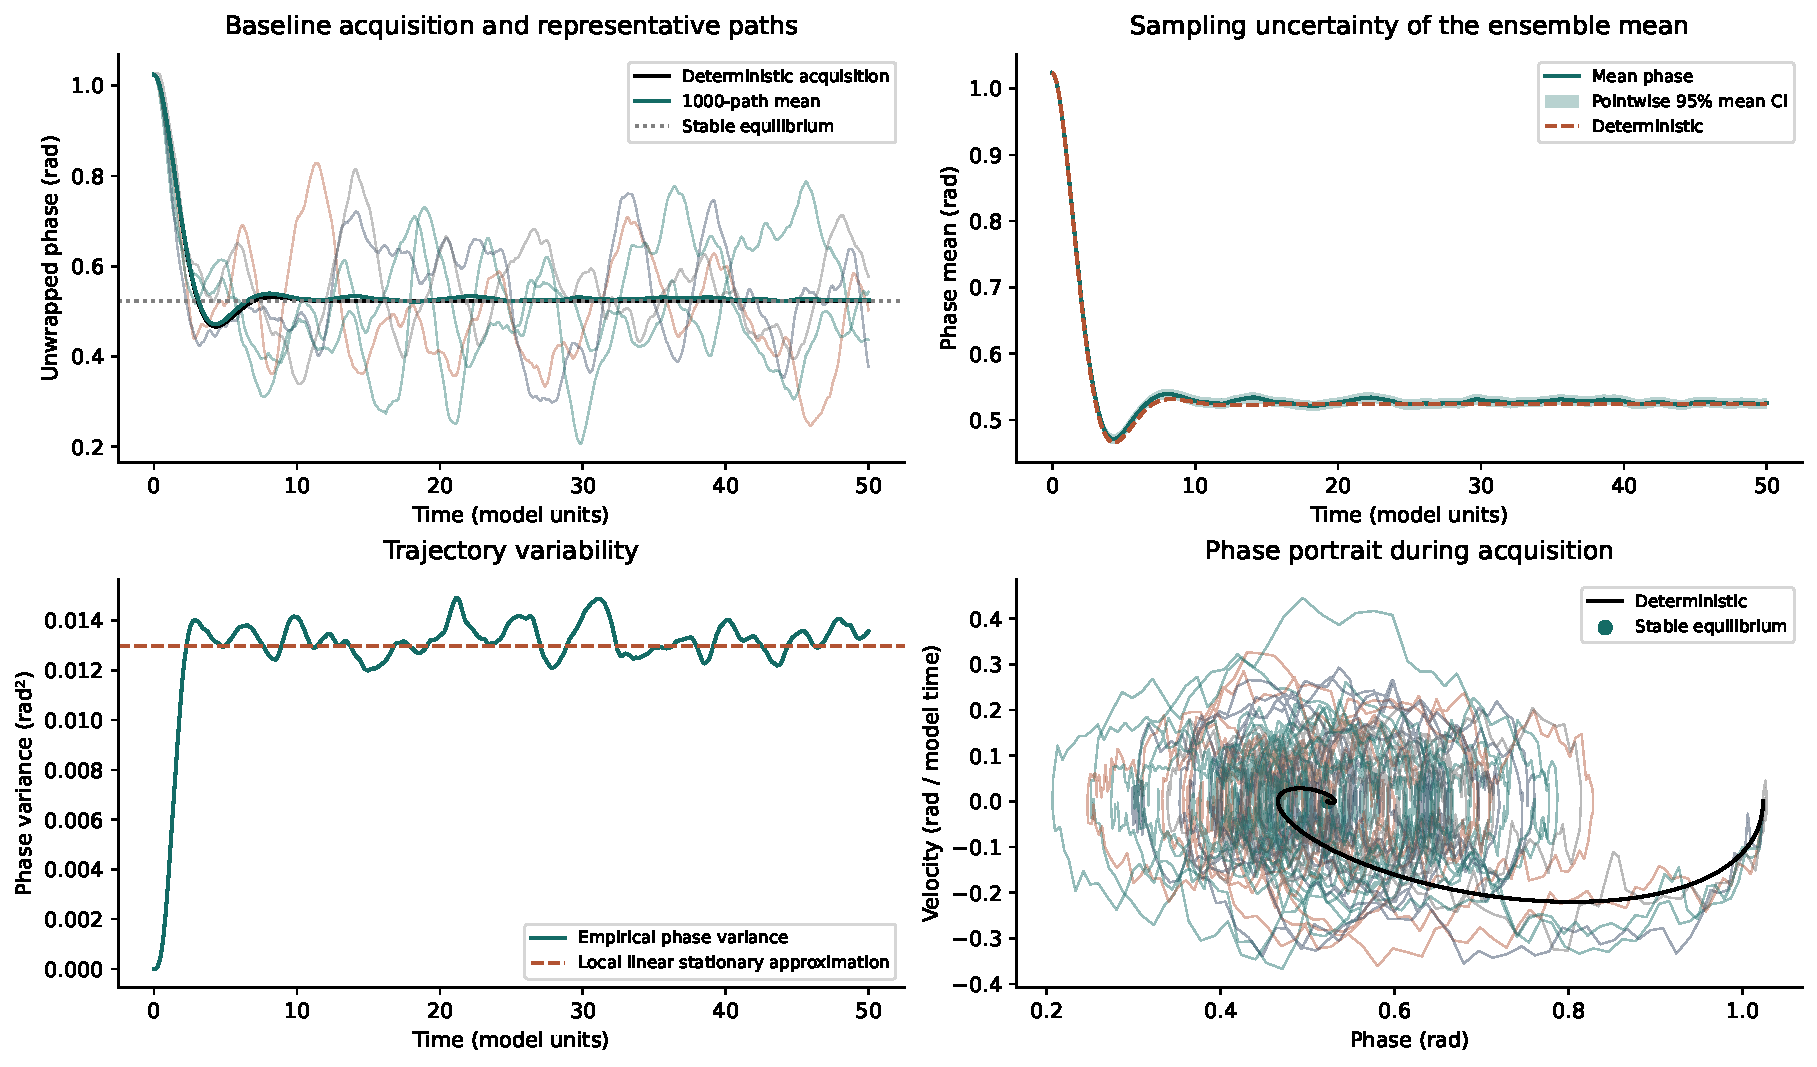
\includegraphics[width=.96\linewidth,height=.38\textheight,keepaspectratio]{figures/baseline.pdf}
\caption{Executed baseline deterministic/stochastic trajectories, ensemble moments and phase-space view. The stable-equilibrium initialization and original acquisition initialization are kept distinct; displayed uncertainty is labeled by its statistical meaning.}
\label{fig:baseline}
\end{figure}
\begin{figure}[htbp]\centering
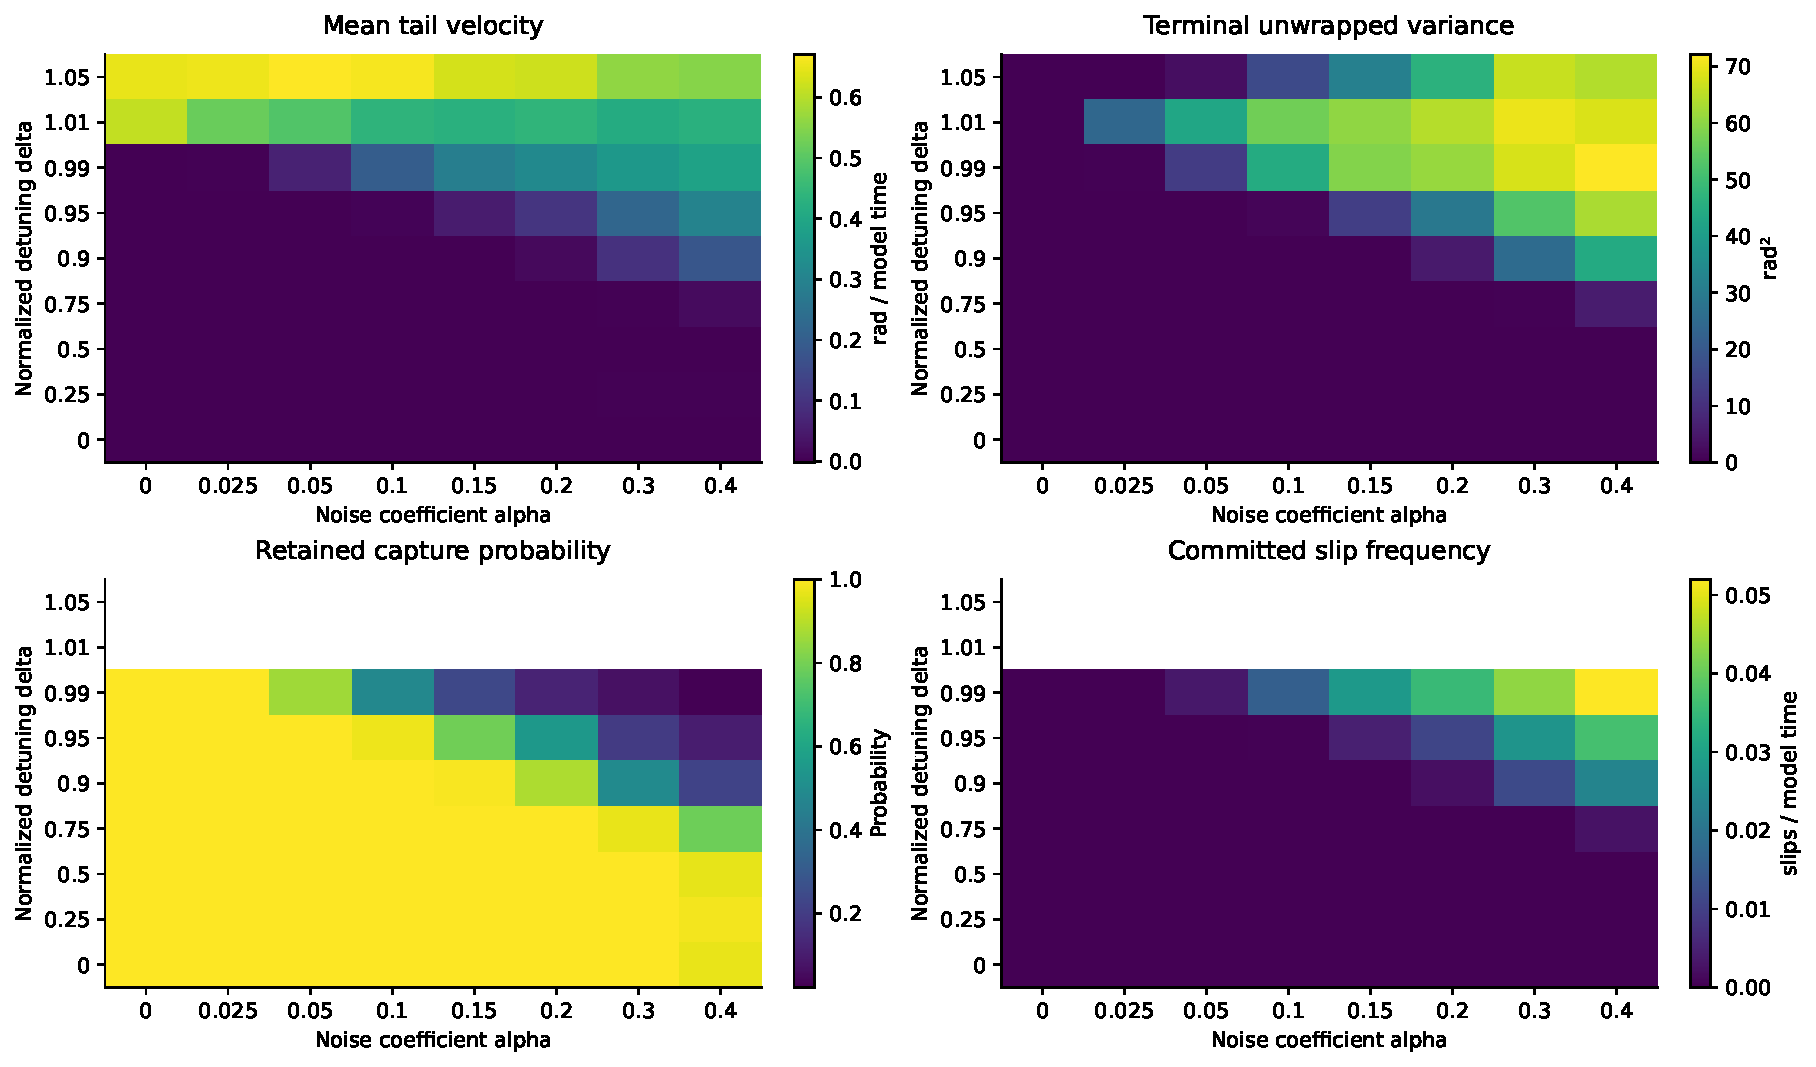
\includegraphics[width=.96\linewidth,height=.38\textheight,keepaspectratio]{figures/combined_grid.pdf}
\caption{Full executed noise--detuning matrix. Near-threshold fluctuations and transitions depend jointly on detuning and noise. Cells without stable equilibria must be interpreted through rotation rather than ordinary locked-state slips.}
\label{fig:grid}
\end{figure}
\begin{table}[htbp]\centering\small
\setlength{\tabcolsep}{4pt}
\begin{tabular}{rrrll}\toprule
$\delta$ & $\alpha$ & $n$ & Tail velocity [CI] & Rotation rate \\ \midrule
1.01 & 0.15 & 500 & 0.425 [0.4, 0.45] & 0.0676 \\
1.05 & 0.15 & 500 & 0.627 [0.608, 0.647] & 0.0999 \\
1.05 & 0.4 & 500 & 0.547 [0.518, 0.577] & 0.0871 \\
\bottomrule\end{tabular}
\caption{Above-threshold dynamics at $T=50$. Tail velocity is in rad/model-time; rotation rate is tail velocity divided by $2\pi$, in cycles/model-time. Equilibrium-based capture and slip columns are not applicable.}
\label{tab:unlocked}
\end{table}
Above threshold, positive mean rotation remains a useful observable while stable-well slip labels cease to apply (Table~\ref{tab:unlocked}). The separate acquisition ensemble has phase variance 0.0136 [0.0123, 0.0148] rad$^2$ at $T=50$ and 0 observed committed slips. Replays of seeds 0--4 and 42 agree with the preserved implementation to maximum phase difference $9.44\!\times\!10^{-16}$ rad and velocity difference $1.05\!\times\!10^{-15}$ rad/model-time. Floating-point roundoff agreement validates recurrence preservation, not the physical noise model.
\subsection{Long horizons, first passage and detector dependence}
\begin{table}[htbp]\centering\small
\setlength{\tabcolsep}{4pt}
\begin{tabular}{rrrrlll}\toprule
$\delta$ & $\alpha$ & Event paths & Slips & Rate [CI] & RMST & Median \\ \midrule
0.75 & 0.15 & 0 & 0 & 0 [0, 0] & 200 & \textemdash \\
0.75 & 0.3 & 65 & 69 & $3.45\!\times\!10^{-4}$ [$2.60\!\times\!10^{-4}$, $4.30\!\times\!10^{-4}$] & 194 & \textemdash \\
0.9 & 0.15 & 49 & 54 & $2.70\!\times\!10^{-4}$ [$1.95\!\times\!10^{-4}$, $3.55\!\times\!10^{-4}$] & 196 & \textemdash \\
0.9 & 0.3 & 934 & 2972 & 0.0149 [0.0142, 0.0155] & 78.2 & 61.4 \\
0.95 & 0.15 & 634 & 1508 & 0.00754 [0.00703, 0.00807] & 132 & 143 \\
0.95 & 0.3 & 998 & 6502 & 0.0325 [0.0317, 0.0333] & 42.2 & 32.2 \\
\bottomrule\end{tabular}
\caption{Long-horizon first-slip and transition statistics: $n=1000$ per row and $T=200$. Rates are committed transitions per trajectory per model time; intervals bootstrap independent path rows. RMST is the restricted mean first-slip time through 200, including right censoring. An unavailable median means survival did not cross one half. Zero-event bootstrap intervals degenerate and require the separate upper bounds discussed in the text.}
\label{tab:long}
\end{table}
At $(\delta,\alpha)=(.95,.15)$, the independent $T=200$ ensemble records 634/1000 paths with a first event and 1508 total transitions. Its restricted mean first-slip time is 132, whereas the mean restricted to observed-event paths is 92.7. The latter omits censored paths and is not the unconditional mean waiting time. Kaplan--Meier survival retains right censoring; no extrapolation beyond 200 is made.

The $(.75,.15)$ long ensemble has no observed events. Its Wilson event-probability upper bound is 0.00383; a separately labeled Poisson exposure approximation gives a rate upper bound $1.50\!\times\!10^{-5}$ per model time. A degenerate zero-event bootstrap interval is not evidence of an exactly zero rate.

At $(.9,.3)$ the primary rate is 0.0149, the loose rate 0.0149, and the strict rate 0.0123. This sensitivity shows that completed recapture and rapid running excursions are distinguished by the detector. The primary detector does not claim to count every engineering notion of a phase slip.
\begin{figure}[htbp]\centering
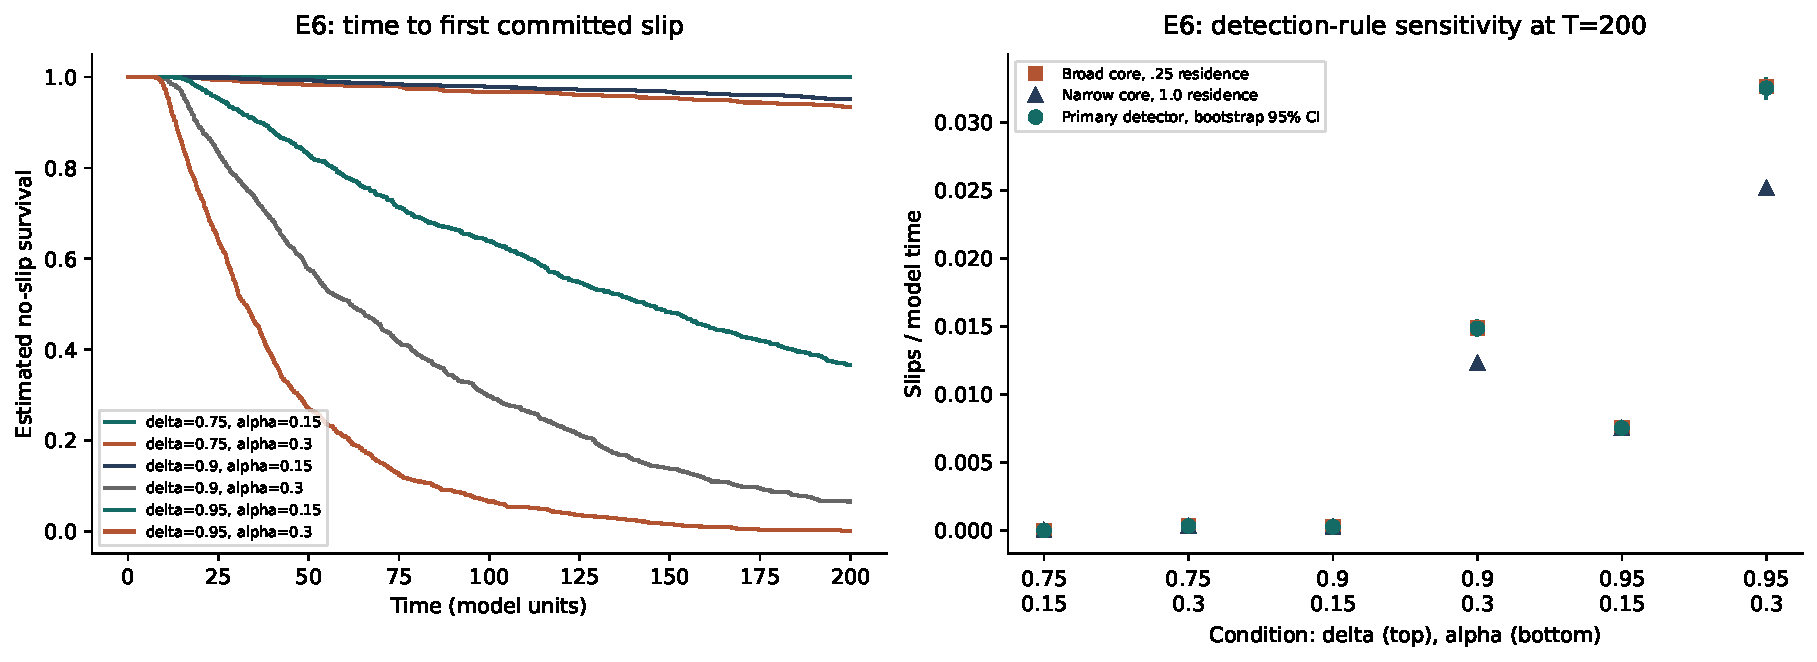
\includegraphics[width=.96\linewidth,height=.38\textheight,keepaspectratio]{figures/slip_survival.pdf}
\caption{Actual long-horizon first-slip survival estimates. Unslipped paths are censored at the horizon; event-time uncertainty and operational detector dependence limit rare-event interpretation.}
\label{fig:survival}
\end{figure}
\subsection{Numerical convergence and parameter sensitivity}
\begin{table}[htbp]\centering\small
\setlength{\tabcolsep}{4pt}
\begin{tabular}{rlll}\toprule
Step $h$ & \shortstack{Baseline RMS\\$\times10^{-3}$ [CI]} & \shortstack{Stress RMS\\$\times10^{-3}$ [CI]} & \shortstack{Stress phase bias\\$\times10^{-3}$ [CI]} \\ \midrule
0.01 & 1.22 [1.18, 1.26] & 12.6 [10.2, 14.9] & -2.14 [-3.11, -1.17] \\
0.005 & 0.601 [0.578, 0.623] & 6.08 [5.04, 7.15] & -1.03 [-1.5, -0.564] \\
0.0025 & 0.293 [0.282, 0.304] & 2.8 [2.35, 3.26] & -0.46 [-0.673, -0.247] \\
0.00125 & 0.138 [0.133, 0.144] & 1.45 [1.18, 1.69] & -0.254 [-0.364, -0.145] \\
0.000625 & 0.0614 [0.0592, 0.0637] & 0.606 [0.506, 0.706] & -0.101 [-0.147, -0.0552] \\
\bottomrule\end{tabular}
\caption{Coupled endpoint state errors relative to the numerical reference $h_{\rm ref}=0.00015625$, $T=10$. All three estimate/interval columns are in units of $10^{-3}$. Baseline: $n=1000$, $(\delta,\alpha)=(0.5,0.15)$; stress: $n=500$, $(0.95,0.4)$. Each state error combines phase and velocity in the declared model units. Intervals quantify Monte Carlo uncertainty, not reference discretization error. Phase bias is a paired weak difference.}
\label{tab:convergence}
\end{table}
All saved convergence states are finite. The fitted log--log endpoint RMS slopes are 1.07 for the baseline and 1.08 for the stress case. These are empirical rates over the tested meshes relative to a finer numerical reference, not exact-solution error certificates. Coarse increments sum the same underlying fine increments, so differences compare discretizations of the same forcing. Weak phase, phase-square and variance differences are stored separately, and no rate is forced on unresolved noisy weak errors. The finite $T=10$ endpoint study does not establish convergence of $T=200$ rare-event rates or of basin boundaries.
\begin{figure}[htbp]\centering
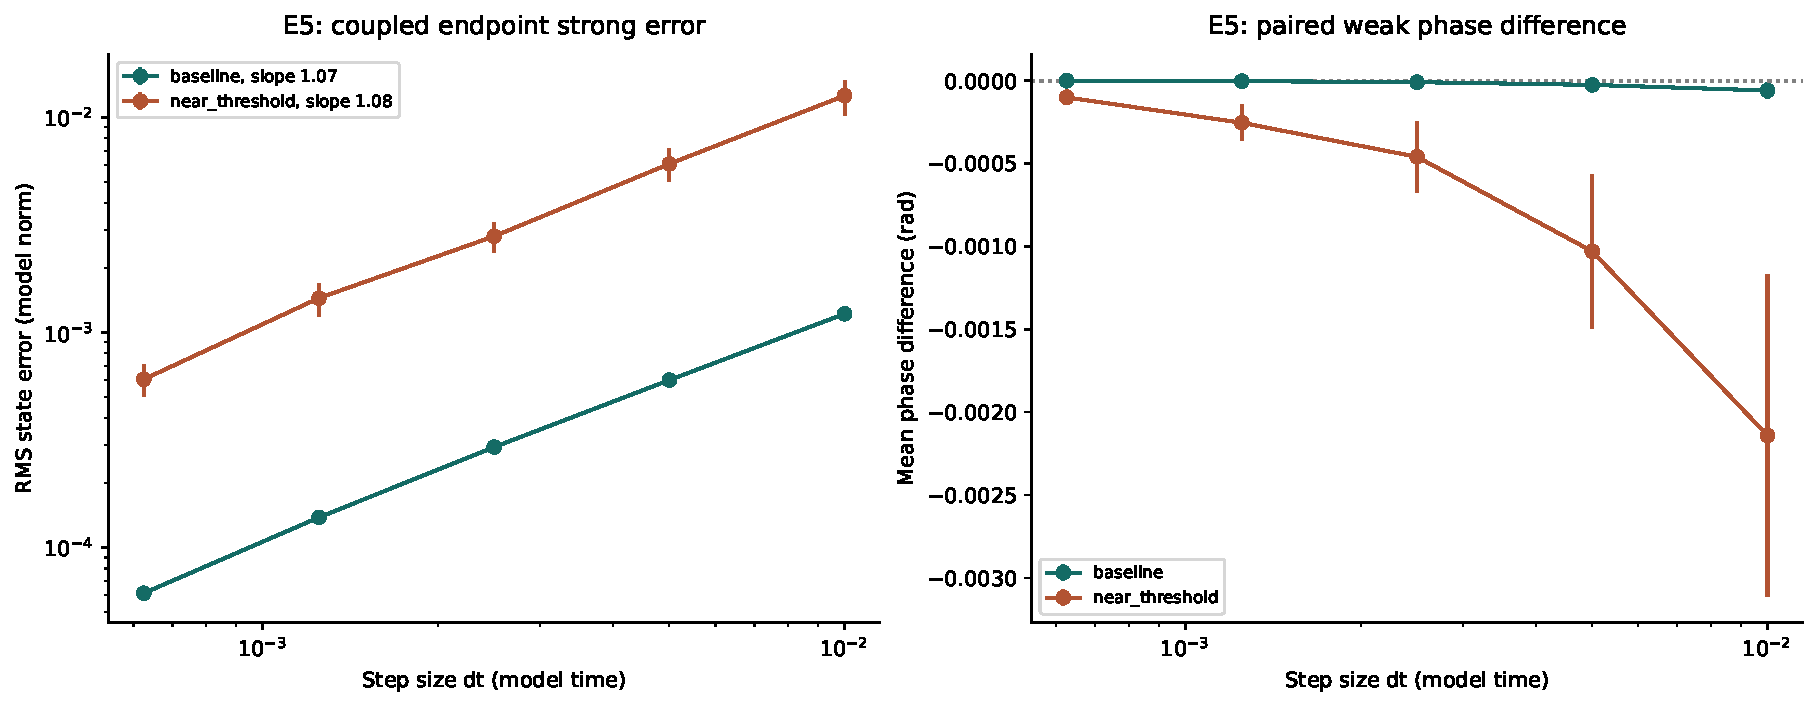
\includegraphics[width=.96\linewidth,height=.38\textheight,keepaspectratio]{figures/convergence.pdf}
\caption{Coupled Brownian mesh comparisons for the baseline and nonlinear near-threshold stress scenario. The reference itself has finite step size; slopes describe the tested error window.}
\label{fig:convergence}
\end{figure}
\begin{table}[htbp]\centering\small
\setlength{\tabcolsep}{4pt}
\begin{tabular}{rrrrrr}\toprule
$a$ & $b$ & $\delta$ & $\widehat{\mathrm{Var}}(\phi_T)$ & Tail velocity & Capture \\ \midrule
0.5 & 0.5 & 2 & 1.16 & 0.452 & \textemdash \\
0.5 & 1 & 1 & 11 & 0.106 & \textemdash \\
0.5 & 2 & 0.5 & 0.013 & $-8.09\!\times\!10^{-4}$ & 1 \\
1 & 0.5 & 1 & 11 & 0.119 & \textemdash \\
1 & 1 & 0.5 & 0.0145 & $7.69\!\times\!10^{-4}$ & 1 \\
1 & 2 & 0.25 & 0.00588 & $-7.79\!\times\!10^{-5}$ & 1 \\
2 & 0.5 & 0.5 & 0.0144 & $-4.69\!\times\!10^{-4}$ & 1 \\
2 & 1 & 0.25 & 0.00569 & $-3.47\!\times\!10^{-6}$ & 1 \\
2 & 2 & 0.125 & 0.00313 & $-8.09\!\times\!10^{-5}$ & 1 \\
\bottomrule\end{tabular}
\caption{E7 at fixed $\Delta=0.5$, $\alpha=0.15$, $n=500$, $T=50$, $h=0.001$. The second noise level $\alpha=0.3$ is also executed and retained in the machine-readable table. Changing $a,b$ changes normalized damping, detuning and noise simultaneously. Dashes denote absence of an ordinary stable well.}
\label{tab:sensitivity}
\end{table}
The E7 results separate no-equilibrium/critical cases from ordinary stable wells. Larger $ab$ at fixed detuning moves the system farther from the equilibrium threshold, while $a$ also changes damping and diffusion in the original units. Consequently the table cannot identify a single standardized causal effect of inertia independently of the other dimensionless groups. The full second noise level and trajectory-level summaries remain available in the CSV/JSON archive.
\subsection{Separately executed synthetic oscillator extension}
The separate synthetic study executes 144 conditions with 72,000 independent network realizations: $N\in\{3,8,20\}$, four topologies, correlation $\rho\in\{0,.5,1\}$, dropout $p\in\{0,.3\}$ and delay $\tau\in\{0,.2\}$. Each uses $T=50$, $h=.01$, coupling 2 and marginal noise amplitude .35. Frequencies are a fixed shuffled grid from $-.5$ to $.5$ and initial phases are independently uniform. Dropout and delay use the separately recorded synthetic protocol; delayed coupling uses stale relative phase error.

\begin{table}[htbp]\centering\small
\setlength{\tabcolsep}{4pt}
\begin{tabular}{rlrrrll}\toprule
$N$ & Topology & $\rho$ & $p$ & $\tau$ & Tail $R$ [CI] & Disagreement \\ \midrule
8 & complete & 0 & 0 & 0 & 0.976 [0.976, 0.977] & 0.0531 \\
8 & ring & 0 & 0 & 0 & 0.945 [0.934, 0.957] & 0.102 \\
8 & star & 0 & 0 & 0 & 0.974 [0.973, 0.974] & 0.0594 \\
8 & sparse & 0 & 0 & 0 & 0.952 [0.95, 0.954] & 0.105 \\
20 & complete & 0 & 0 & 0 & 0.974 [0.974, 0.974] & 0.0539 \\
20 & ring & 0 & 0 & 0 & 0.458 [0.445, 0.471] & 0.805 \\
20 & star & 0 & 0 & 0 & 0.973 [0.973, 0.974] & 0.0554 \\
20 & sparse & 0 & 0 & 0 & 0.767 [0.761, 0.773] & 0.426 \\
3 & complete & 0 & 0 & 0 & 0.983 [0.983, 0.983] & 0.0504 \\
20 & complete & 1 & 0 & 0 & 0.989 [0.989, 0.989] & 0.0224 \\
8 & ring & 0.5 & 0 & 0 & 0.897 [0.876, 0.919] & 0.153 \\
8 & ring & 1 & 0 & 0 & 0.785 [0.752, 0.817] & 0.28 \\
20 & sparse & 0 & 0.3 & 0.2 & 0.595 [0.582, 0.609] & 0.641 \\
20 & sparse & 0.5 & 0.3 & 0.2 & 0.62 [0.606, 0.634] & 0.609 \\
20 & sparse & 1 & 0.3 & 0.2 & 0.674 [0.658, 0.69] & 0.514 \\
\bottomrule\end{tabular}
\caption{Selected synthetic network results, $n=500$ networks per row. Tail summaries use $t\ge40$. Intervals for tail $R$ are Student-based across independent networks. Disagreement is the tail mean of pairwise $1-\cos(\theta_i-\theta_j)$. The three-agent ring and complete graph have identical adjacency, so they are not distinct topology evidence.}
\label{tab:synthetic}
\end{table}
For the 20-agent complete graph without dropout/delay, tail concentration is 0.974 for independent noise and 0.989 for shared noise. Shared additive noise cancels exactly in phase differences: increasing correlation reduces differential noise at fixed marginal amplitude, rather than intrinsically synchronizing uncoupled agents. Topology comparisons depend on the degree-normalization convention and the specified frequency grid. These synthetic measurements assess oscillator coordination, not language-model correctness or communication-token savings.
The eight-agent clean ring is a counterexample to a monotone correlation--concentration interpretation: tail $R$ is 0.945 at $\rho=0$ and 0.785 at $\rho=1$, while tail frequency dispersion falls from 0.0287 to $1.13\!\times\!10^{-7}$. Low global concentration can therefore coexist with near-equal frequencies and a nonuniform locked phase profile. Diagnostic replays of existing paths investigate winding states; they are not counted as extra independent trajectories.
\subsection{Reproducibility and limitations}
The preflight record reports \texttt{25 passed in 1.70s}. The full post-run test record reports \texttt{38 passed in 13.48s}. Checks cover reproducibility, Brownian scaling, deterministic agreement, equilibrium classification, finite states, completed transitions and statistical calculations. The execution manifest, source fingerprints, per-condition configuration, seeds, trajectory rows and sampled paths are preserved. The recorded environment uses Python 3.14.8, NumPy 2.5.0, SciPy 1.18.0, pandas 3.0.4 and Matplotlib 3.11.0. Master seed 20261113 and condition/trajectory identifiers initialize independent reproducible streams.

From the project root, execute \texttt{python -m src.reproduce}; \texttt{--reports-only} regenerates reports from saved results. The individual validation command is \texttt{python -m pytest -q}; granular workflows are documented in \texttt{README.md}. The formal report is rebuilt by \texttt{python -m src.latex\_report}; compile inside \texttt{report/} using \texttt{tectonic main.tex}, or two \texttt{pdflatex main} passes with the required packages installed. Its explicit bibliography is generated from the eleven verified reusable \texttt{references.bib} records, so a separate BibTeX executable is unnecessary. The HTML report contains the extended derivations and code walkthrough; this concise report retains the scientific model, measured results and their limits.

The principal limits are synthetic rather than measured input, uncalibrated time/noise, finite horizon and sample size, operational detector thresholds, a finite numerical reference, and no proof of global capture or rare-event asymptotics. Pointwise and per-cell intervals do not supply familywise simultaneous confidence. Comparisons are descriptive and mechanism-informed; no unsupported novelty or significance claim is made.

\section{Conclusion and Possible Extensions}
The textbook equation supports a reproducible, statistically explicit study that goes beyond a few noisy traces. The saved ensembles distinguish small local fluctuations from large unwrapped displacements, show why near-threshold and longer-horizon studies matter, and separate above-threshold rotation from equilibrium-based slips. Standard Milstein and Euler--Maruyama coincide for this additive-noise model; coupled results support approximately first-order endpoint behavior over the tested meshes without proving rare-event convergence.

Further work should calibrate a physical loop and noise spectrum, validate event definitions against application-specific requirements, compare higher-order/integrated-noise methods, and resolve very rare transitions with justified longer horizons or validated rare-event algorithms. A synthetic oscillator network is a separate mathematical extension. LLM communication requires an independently validated coordination signal, full benchmark controls and approved costs before any claim about reasoning performance. No physical phase interpretation or benchmark improvement follows from synchronization alone.

\clearpage
\begin{thebibliography}{11}
\bibitem{kloeden1992} Kloeden, Peter E.; Platen, Eckhard. \emph{Numerical Solution of Stochastic Differential Equations}. Springer, 1992. \url{https://doi.org/10.1007/978-3-662-12616-5}.
\bibitem{higham2001} Higham, Desmond J. An Algorithmic Introduction to Numerical Simulation of Stochastic Differential Equations. \emph{SIAM Review}, \textbf{43}(3), pp.~525--546 (2001). \url{https://doi.org/10.1137/S0036144500378302}.
\bibitem{bobrovsky1982} Bobrovsky, B. Z.; Schuss, Z. A Singular Perturbation Method for the Computation of the Mean First Passage Time in a Nonlinear Filter. \emph{SIAM Journal on Applied Mathematics}, \textbf{42}(1), pp.~174--187 (1982). \url{https://doi.org/10.1137/0142014}.
\bibitem{bianchi2015} Bianchi, G.; Kuznetsov, N. V.; Leonov, G. A.; Yuldashev, M. V.; Yuldashev, R. V. Limitations of {PLL} Simulation: Hidden Oscillations in {MatLab} and {SPICE}. In \emph{2015 7th International Congress on Ultra Modern Telecommunications and Control Systems and Workshops (ICUMT)}, pp.~79--84 (2015). \url{https://doi.org/10.1109/ICUMT.2015.7382409}.
\bibitem{kramers1940} Kramers, H. A. Brownian Motion in a Field of Force and the Diffusion Model of Chemical Reactions. \emph{Physica}, \textbf{7}(4), pp.~284--304 (1940). \url{https://doi.org/10.1016/S0031-8914(40)90098-2}.
\bibitem{khasminskii2012} Khasminskii, Rafail. \emph{Stochastic Stability of Differential Equations}. Springer, 2nd edition, 2012. \url{https://doi.org/10.1007/978-3-642-23280-0}.
\bibitem{acebron2005} Acebr{\'o}n, Juan A.; Bonilla, L. L.; P{\'e}rez Vicente, Conrad J.; Ritort, F{\'e}lix; Spigler, Renato. The {Kuramoto} Model: A Simple Paradigm for Synchronization Phenomena. \emph{Reviews of Modern Physics}, \textbf{77}, pp.~137 (2005). \url{https://doi.org/10.1103/RevModPhys.77.137}.
\bibitem{li2024} Li, Yunxuan; Du, Yibing; Zhang, Jiageng; Hou, Le; Grabowski, Peter; Li, Yeqing; Ie, Eugene. Improving Multi-Agent Debate with Sparse Communication Topology. In \emph{Findings of the Association for Computational Linguistics: EMNLP 2024}, pp.~7281--7294 (2024). \url{https://doi.org/10.18653/v1/2024.findings-emnlp.427}.
\bibitem{cobbe2021} Cobbe, Karl; Kosaraju, Vineet; Bavarian, Mohammad; Chen, Mark; Jun, Heewoo; Kaiser, Lukasz; Plappert, Matthias; Tworek, Jerry; Hilton, Jacob; Nakano, Reiichiro; Hesse, Christopher; Schulman, John. Training Verifiers to Solve Math Word Problems. \emph{arXiv preprint arXiv:2110.14168} (2021). \url{https://doi.org/10.48550/arXiv.2110.14168}.
\bibitem{gsm8krepository} {OpenAI}. \emph{Grade School Math: Official {GSM8K} Repository}. GitHub repository. Accessed 13 November 2026. \url{https://github.com/openai/grade-school-math}.
\bibitem{wang2026} Wang, Boxuan; Li, Zhuoyun; Huang, Xiaowei; Dong, Yi. Do We Need Complex Topology Control? Distinct-Peer Random Routing Improves Cost-Efficiency in Sparse Multi-Agent Debate. \emph{arXiv preprint arXiv:2609.27150} (2026). \url{https://arxiv.org/abs/2609.27150}.
\end{thebibliography}
\end{document}
